\documentclass[11pt,a4paper]{report}

\UseRawInputEncoding
\usepackage{url}
\usepackage{hyperref}
\usepackage[utf8]{inputenc}
\usepackage{graphicx}
\usepackage[all]{xy}
\usepackage{amsmath}
\usepackage{amsthm}
\usepackage{todonotes}
\usepackage{array}
\usepackage{listings}
\usepackage[a4paper]{geometry}
\usepackage{float}
\usepackage[english]{babel}
\usepackage[nottoc]{tocbibind}
\usepackage[square,numbers]{natbib}


\usepackage{filecontents}
\begin{filecontents*}{mystyle.sty}
\NeedsTeXFormat{LaTeX2e}
\ProvidesPackage{mystyle}
\newenvironment{acknowledgments}
  {\renewcommand{\abstractname}{Acknowledgments}% Abstract > Acknowledgements
   \begin{abstract}}
  {\end{abstract}
   \clearpage}
\endinput
\end{filecontents*}
\usepackage{mystyle}

\makeatletter %otherwise geometry resets everything
\Gm@restore@org
\makeatother

\setlength{\itemsep}{0cm}
\setlength{\voffset}{0cm}
\setlength{\headheight}{0cm}
\setlength{\topmargin}{0cm}
\setlength{\marginparwidth}{2cm}
\setlength{\extrarowheight}{3pt} %for superscripts in tabular
\setlength{\arraycolsep}{4pt}
\lstset{basicstyle = \footnotesize, breaklines = true}

\graphicspath{{imgs/}}

\begin{document}
\begin{titlepage}
\begin{center}
\textsc{\LARGE Master thesis}\\[1.5cm]

\includegraphics[height=100pt]{tbs_logo_2019.png}

\vspace{0.4cm}
\textsc{\Large Toulouse Business School}\\[1cm]
\hrule
\vspace{0.4cm}
\textbf{\huge Classifying Short Text for \\Harmonized System with \\Google BERT\\[0.3cm]
\LARGE }
\hrule
\vspace{2cm}
\begin{minipage}[t]{0.52\textwidth}
\begin{flushleft} \large
\textit{Author:}\\
Kevin Darmon\\
\texttt{k.darmon@tbs-education.org}\\[1.3cm]
\end{flushleft}
\end{minipage}
\begin{minipage}[t]{0.45\textwidth}
\begin{flushright} \large
\textit{First supervisor/assessor:}\\
Prof.dr. Kevin Carillo\\
\texttt{k.carillo@tbs-education.fr}\\[1.3cm]
\textit{Second assessor:}\\
Olivier Mallet\\
\texttt{olivier.mallet@atos.net}
\end{flushright}
\end{minipage}
\vfill
{\large \today}
\end{center}
\end{titlepage}

\begin{abstract}
Automatic text classification is an active field of research over the last decades due to the rapid growth of online documents. As a consequence, several scientific publications provide an overview of current classification techniques. The general trend of these publications is that several Machine Learning techniques make progress in text classification problems. Common research areas within text classification are topics, emails, and sentiment classification. \\ 
\\
The general approach in these tasks is similar in extracting the meaning of the text (features) to find the appropriate class or label. However, the results of these techniques depend on to which extent a technique is able to model the underlying structure of the documents that belong to labels. In this process, a variety of techniques, combined with a mixture of parameters are chosen in order to model a classifier. Finding suitable structures, architectures, and techniques for text classification is, in particular, a challenge for researchers.\\
\\
Therefore, in this thesis, i will be focussing on applying state-of-the-art technics Google BERT, which is using a pre-trained model to tackle NLP problematics and can be used in many different languages (103 actually). As shown by \citeauthor{Devlin2018}. , BERT can be easily fine-tuned to be part of every project. Nonetheless, it as not been shown that BERT could handle short text and/or word for classification. 
\end{abstract}

\begin{acknowledgments}
This thesis project owes a great deal to Atos, as without their knowledge, data and ressources, this project would not have been possible. \\
\\
I would like to thank a number of people at Atos in particular. First and foremost, my manager, Olivier Mallet, for his support and encouragements, also for matching me with this project and giving me the opportunity to work at a high level, and even allowing me to present my work in front of a large group of the expert community at Atos. Additionally, I would like to thank Yaroslav Logachev for his domain expertise and insights. A special thanks also to my team, for helping me with this project and sharing their knowledge and help me troubleshoot all of my problem.\\
\\
Lastly, I’d like to thank Kevin Carillo, my supervisor, without his guidance and inspiration I would not have been able to complete this thesis. Kevin, you’ve been one of the most approachable and friendly professors I’ve met, and I hope you continue to share that kindness with your students.
\end{acknowledgments}
\tableofcontents
\UseRawInputEncoding
\chapter{Introduction}\label{ch:intro}
\section{General Introduction}
The world increasingly relies on logistic processes to supply and provide for
an ever-growing population. Facilitating global trade is a shared customs
standard that classifies goods with a numerical code, allowing every customs
authority to implement the same nomenclature. This standardized
system is the Harmonized System (HS) which classifies goods in a hierarchical
code framework. These codes appear on standard freight documents
such as waybills and Single Administrative Documents (SAD). At the core
of these documents is a provision for a textual description of goods. An
example of a description alongside a valid HS code is shown in 1.1. The
burden of providing the correct code and valid text description is placed
on the trader, who has to supply and ascertain that both of these are correct.
However, due to the complexity of the system this classification process
remains hard to do for non-experts, with some agencies estimating a rate of
misclassification of between 17(\%) and 30(\%) \cite{OfficeoftheAuditorGeneralofCanadaGovernmentofCanada.2010}. More detailed information
on the Harmonized system itself and the consequences of miss-classification
can be found in the last section of this chapter. \\

\begin{center}
    \begin{tabular}{lc} \hline \centering
Description & HS Code \\ \hline
Parts of filtering or purifying machinery & 842199 \\ \hline
	\end{tabular}
\end{center}
{\textit{Table 1.1: An example of a (corrected) HS-classification. The HS code shown here is defined at the HS-6 level, which defines over 5000 possible labels.}} \\

Classification on the basis of these texts to find the correct HS label is a complex problem, due to a number of problems:
\begin{itemize}
\item The textual descriptions are brief, creating a sparse feature space for classification
\item These descriptions do not follow natural language syntax and often lack the structure otherwise found in text
\item The number of possible labels for a text description is rather large compared to other text classification problems, at over 5000 at the highest level of detail
\item Keywords such as ”diesel fuel” that may be used to identify a product appear both when defining a raw form of the item, as well as parts of products such as waxes or engines (”diesel engine”), or even when describing complete vehicles
\item Not all product labels are as frequent as others, making it hard to gather data on edge cases
\item Misspellings and grammatical errors are common \cite{Li2016} and are hard to correct without more context
\item The text descriptions often contain special domain-specific words specific to shipping, such as the abbreviations stc, “said to contain”, and fcl, which stands for “full-container load”
\item The occurrence of Hapax legomena, words or phrases, or even complete descriptions, that only appear once, is frequent.
\end{itemize}

In order to attempt to provide a computational solution to this problem we focus on the use of a state of the art Natural Language Processing (NLP) model Google BERT, a deep neural networks technique for text classification introduced by \cite{Devlin2018}, which since his introduction is the new standards as a base model for new NLP model. \\


\section{Research Focus}
In this work, we aim to classify goods descriptions on the HS-2 and HS-4 level. While the HS-2 level is arguably high-level and has, therefore, limited use for customs purposes, the HS-4 level sees significant use in summary declarations. However, at this time of writing this thesis research, work has not been done with the HS-2 level. So for the rest of this current version of the thesis, i will talk about both but only demonstrates my approach with the HS-2 level.

Our main research question is formulated as follows: can we apply the state of the art NLP model Google BERT to classify HS codes based on short descriptions? For this, i will describe my methodology on how I pre-process the data all the way to the result.\\


Neural networks for natural language processing have experienced a surge in popularity in recent years. The most common methods can be roughly grouped into two categories: Convolutional Neural Networks and Recurrent Neural Networks (which include Long-Short-Term Memory (LSTM) networks and Gated Recurrent Units (GRUs)).\\


Recurrent neural networks are not an odd choice, as they excel with modeling sequential data. They have been utilized for language model problems and have in general been applied with success \cite{Mikolov2010a, Chung2014, Lai2015, Howard2018, Xu}. However, they were initially not well-suited to deal with correlations that are further apart in sentences, due to the vanishing gradient problem during back-propagation where the gradient propagated through the network becomes close to zero when more time steps are made.\\


Current approaches also include bi-directional LSTMs, which pass over text both from left-to-right and right-to-left. This greatly enhances the ability of RNNs to deal with longer dependencies in text. Among these, the ELMo model \cite{Peters2018} successfully applies this concept to produce embeddings that change on differing sentences (context).\\
Attention mechanisms are also popular and are currently popular choices to capture dependencies in text \cite{Lin2017, Openai}. One specific attention mechanism is the transformer, an encoder-decoder architecture that involves an attention mechanism to capture dependencies in text \cite{Vaswani2017}. BERT \cite{Devlin2018} successfully combines this idea with a Masked Language Model objective to produce a complex language model that can be applied to many downstream tasks. It is worth noting that the concept of pre-training on outside data and applying a trained model to supervised tasks is still adhered to with these models. However, with these developments it seems that the concept of transfer learning in language models is definitely shifting from mere word embeddings to more sophisticated models that have been trained for a long period of time, which is very much like the trend in computer vision.\\


Lastly, it is possible to forsake word-level embeddings completely and construct a convolutional neural model based on characters \cite{Zhang2015, Conneau2017, Shrestha}. These models rival the performance of word-embedding CNNs, but despite their elegance require a deeper network and a larger training time budget \cite{Le2017, Conneau2017, Adams2018}.

\newpage
\section{Background: The Harmonized System}
Nowadays, customers are used to buying and ordering products all over the world with only a few clicks on the web. Products are exported and shipped all over the world and these arrive in only a couple of weeks or even days at their destination. This scenario illustrates the enormous increase in global trading over the last decades \cite{EstebanOrtiz-Ospina2018} and even years \cite{World-Trade-Statistical-2018}. To facilitate this massive global trading there is a need for a common basis that identifies products. The World Customs Organisation (WCO) has published the ‘language of trade’ by means of the Harmonized System (HS) \cite{GeneralSecretariatoftheWorldCustomsOrganisationWCO1983, Chan2015} , which is a nomenclature to classify goods. The Harmonized System is a complex hierarchical system, with multiple levels that divide goods into chapters, headings, and finally subheadings. While the top-most level only contains up to 99 definitions, the system allows for over 5300 precise definitions at the level of subheadings. 
When the customs authorities are given a product, they classify this to a label that corresponds to that type of product. The label of the product uniquely identifies a product. This is important for governments in terms of the calculation of duties, taxes, and fees; determination of permits, license and certificates required and the collection of trade statistics \cite{Ding2015}. Furthermore, countries have the full liberty to extend upon subheading definition with one or two more levels for their own internal needs \cite{Weerth2008}. Examples of these extensions are the Brazilian NCM and the United States’ HTS. It is important to note that at every level the system is defined by both a code and a textual description and that at each level the definitions become more detailed. In this way, the Harmonized System works as a common basis facilitating trade across more than 200 countries all over the world.\\

Current reports have shown that classifying goods and products according to the Harmonized System is a difficult task. According to the Customs duty of Canada, one out of five goods is incorrectly classified \cite{AuditorGeneralofCanada2017}. Besides, it was estimated that the government of Canada missed approximately 21 million dollars due to misclassification in a single year \cite{AuditorGeneralofCanada2017}. A large IT company (Atos) has the information that authorities have employees that classify goods working 120 FTE (Full-time equivalent) per week. Misclassification can occur due to the high number of possible labels, confusing and extensive descriptions of products and the enormous amount of goods to be classified \cite{Kappler2011a}. With this all in mind a way to automatically classify goods can be highly beneficial to the entire process of classification.\\

In the current thesis, research is conducted on an automatic classification of products on a large amount of classes. A large IT company has provided a dataset containing a wide range of products. This dataset is a collection of descriptions of a product and their corresponding HS-code. Rather than complete English sentences these descriptions contain a collection of keywords of the products. Therefore, this research involves experiments of classification on short texts of products. In the field of Natural Language Processing this task is often referred to as text classification in which a document is assigned to classes or categories \cite{Manning2008}. Examples are identifying spam emails and sentiment classification of tweets or reviews.\\

Previous research into an automatic classification of HS codes rendered promising results in classifying goods \cite{Ding2015} \cite{Li2019}. In these recent studies, the authors achieve a high accuracy score ( \textgreater 0.9) in classifying the actual product. However, the task is only carried out on a portion of the labels. In Ding et al. \cite{Ding2015} only chapters 22 and 90 were selected because these chapters were most likely to be misclassified in practice. In Li et al. \cite{Li2019} descriptions and images of four classes were selected because classification on all classes was considered extremely difficult. By reducing the number of classes taken into account, both types of research heavily reduced the complexity of the problem. Nevertheless, to the best of knowledge, text classification of HS codes with a high number of products has not been done before. Moreover, in this thesis, images of products are not available; as a consequence, the authors only focus on classification based on text. Text classification is an active field of study including topic, \cite{Liu2016}, email \cite{7921698} and sentiment \cite{doi:10.1146/annurev-linguistics-011415-040518} classification. 

\subsection{Examples}
In the Harmonized System, a sand-moving diesel-fuel using bulldozer falls under the chapter of nuclear reactors, boilers, machinery, and mechanical appliances, or parts thereof. This chapter has code 84. One level lower is the description of self-propelled bulldozers, angledozers, graders, levelers, scrapers, mechanical shovels, excavators, shovel loaders, tamping machines, and road rollers. The harmonized system code description for this heading is 8429. The system then still goes deeper when defining the subheading group of self-propelled bulldozers and angledozers other than track-laying. This description matches the code 842919. Countries are allowed to extend this system with their own codes, which are added as a suffix to the subheading code (HS-6). This is illustrated in table 1.2.

\begin{center}
    \begin{tabular}{lccccc} \hline \centering
Level & Example Code \\ \hline
Chapter (HS-2) & 84\\
Heading (HS-4) & 8429\\
Subheading (HS-6) & 842919\\
Country-specific extension (HS-8 and beyond) & 84291900\\ \hline
\end{tabular}
\end{center}
{\textit{table 1.2: The hierarchical nature of the Harmonized System demonstrated}} \\

For the sake of consistency, we will refer to these descriptions according to the length of their corresponding HS-code. Thus, the chapter will be referred to as HS-2, the heading as HS-4, and the subheading as HS-6. In the case of country-specific data with a code consisting out of 8 digits, we will refer to these as HS-8. While the classification system includes 21 sections as well as a super-group of chapters, this is outside of the scope of this research as these are not tied to the Harmonized System’s code itself and have limited relevance for classification.

\subsection{Usage of the Harmonized System}
Upon entering a country, carriers are required to present a customs form for their cargo. An example of such a form is shown in 1.1, with the fields for product descriptions marked. Other countries or customs unions have their own forms, but the general usage is, due to the high degree of adaption of the harmonized system, essentially the same. This form contains information on the shipment and is often the first item considered when evaluating which shipments should be inspected if it so happens that doubts are raised regarding the truthfulness of the declaration. The form specifically has fields for a text describing the cargo and its corresponding classification, written by traders or agents.
\\

Another example of an HS-code as it is likely to appear in its use for the consumer market can be seen in Figure 1.2. This sticker includes a European Combined Nomenclature (CN) subheading code of eight digits (HS-8) along with a product description. Interestingly, the code consists of eight digits. This means that we can infer that the product was imported from inside the EU, as imports from outside the EU are given a TARIC code (corresponding to HS-10) instead.\\

Lastly, HS classification codes serve as a way to collect statistics on what is imported and exported to a country. Although this is a significant focus of the Harmonized System, it is outside of the scope of this thesis.

\begin{figure}
    \centering
    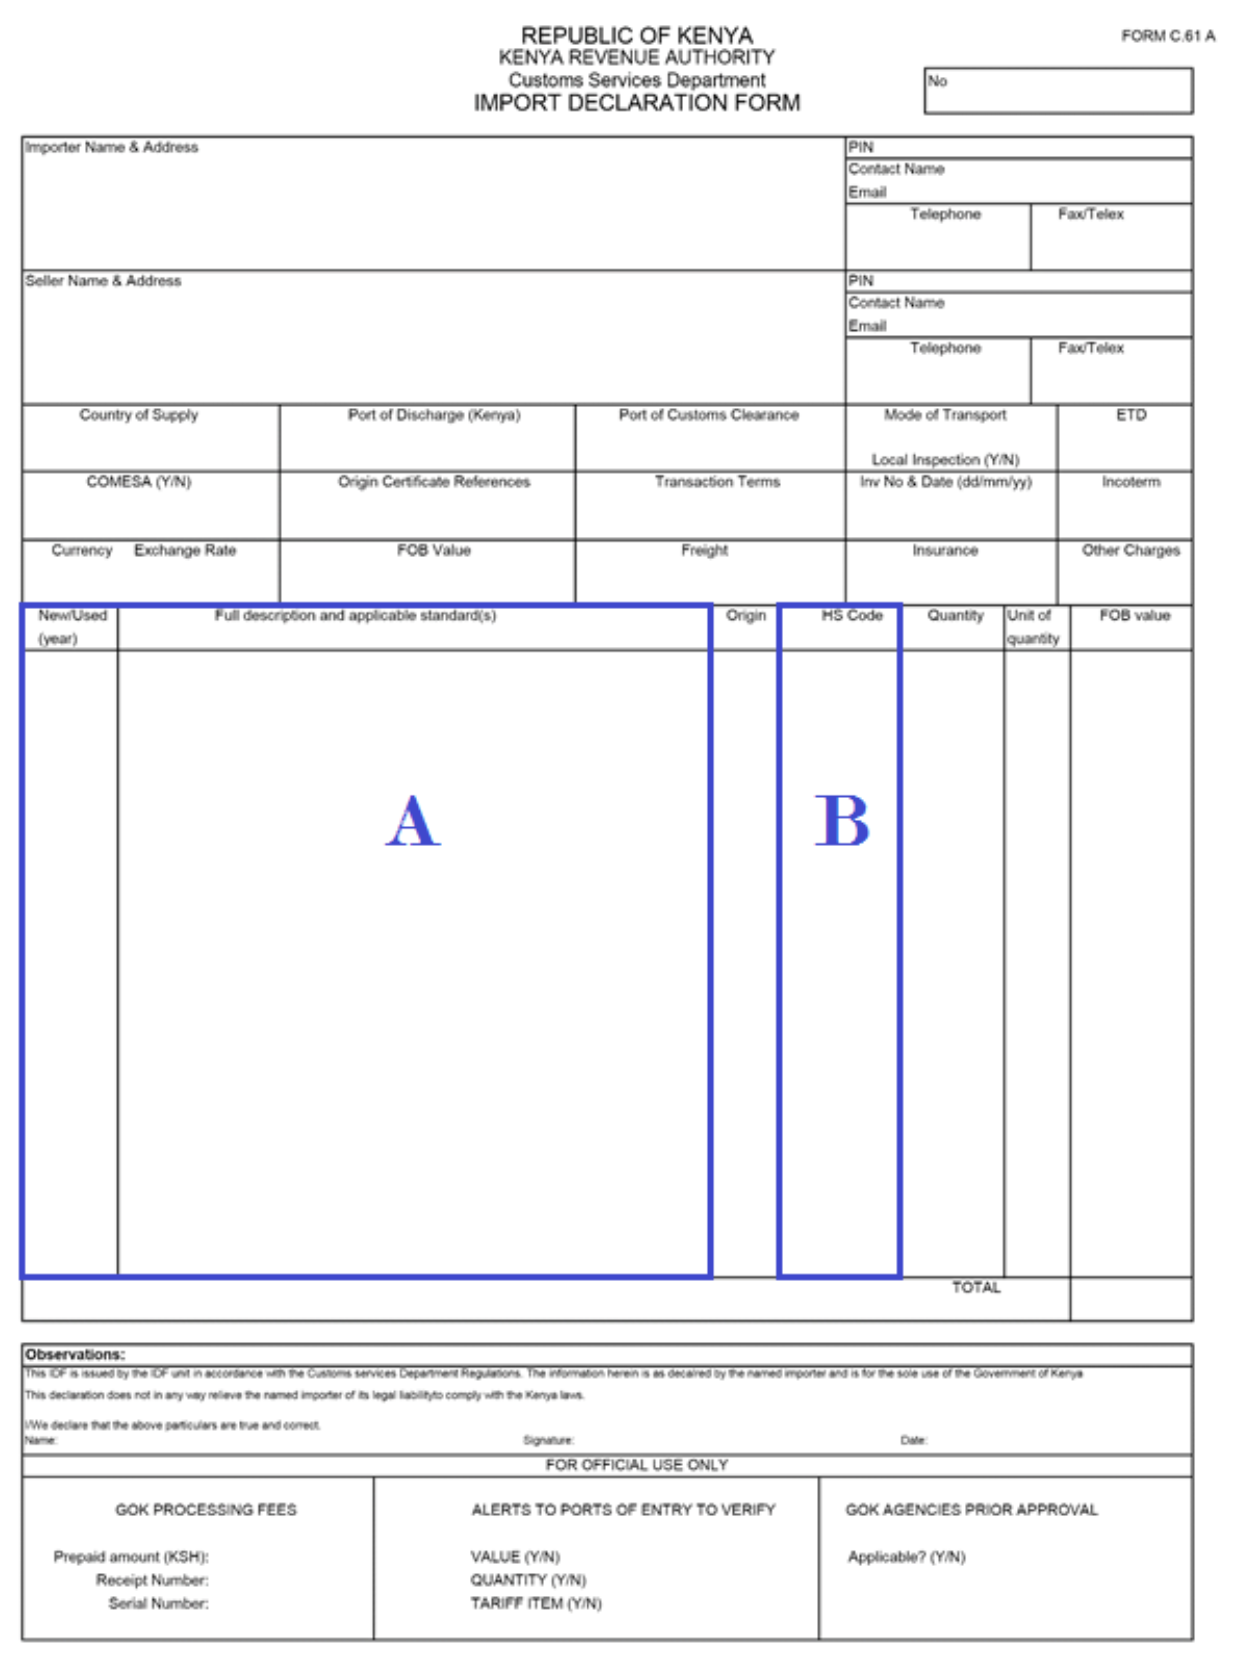
\includegraphics[width=0.8\textwidth]{kenya.png}
    \caption{The Kenyan customs form 61a, which is used to declare imports. Outlined are two relevant sections to describe products and assign a HS- code. Forms like these are used world-wide. Section A provides a text field for a product description, and section B provides a field for the HS code. Other fields on the form are not used within this thesis, but one could argue they can easily be utilised to improve performance on classification tasks.}
    \label{fig:kenya}
\end{figure}


\begin{figure}
    \centering
    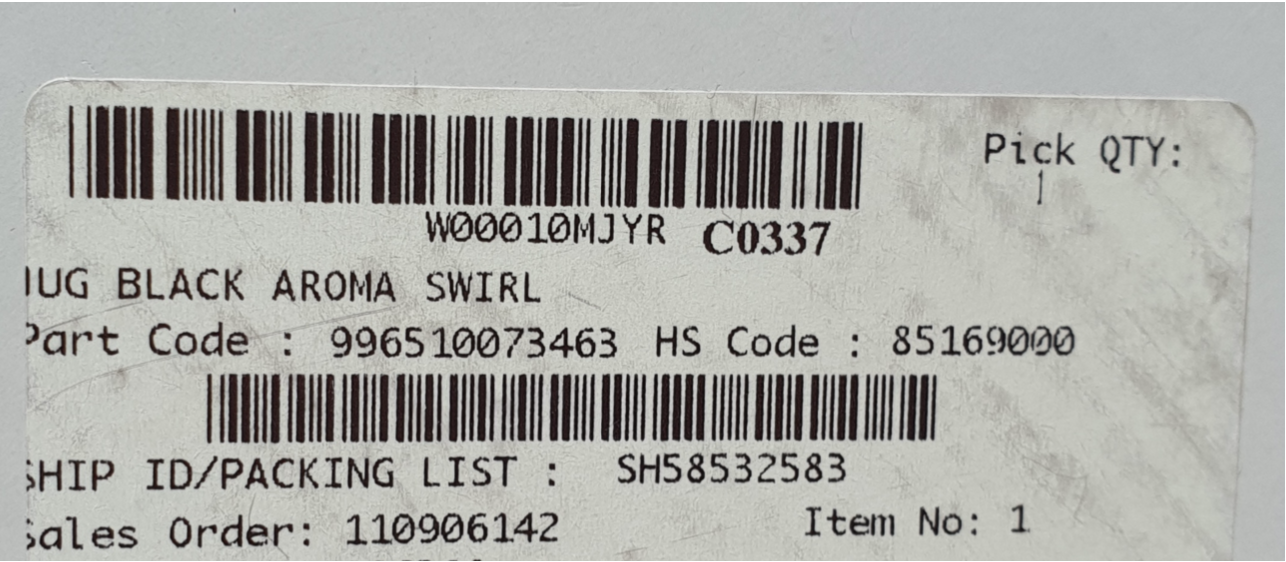
\includegraphics[width=0.8\textwidth]{sticker.png}
    \caption{A HS code as it is likely to appear with documents accompanying packages. This sticker contains a textual description (‘JUG BLACK AROMA SWIRL’) and a HS-8 code (85169000) which corresponds to parts of electric instantaneous or storage water heaters and immersion heaters; electric space-heating apparatus and soil-heating apparatus; electrothermic hairdressing apparatus (for example, hairdryers, hair curlers, curling tong heaters) and hand dryers; electric smoothing irons; other electrothermic appliances of a kind used for domestic purposes; electric heating resistors, other than those of heading 8545. The item imported was a coffee pot.}
    \label{fig:stickers}
\end{figure}


\chapter{Related Work}\label{ch:rel}

In 2016 Han Veiga and Eickhoff collected a dataset of 850 authentic English-speaking users across Twitter, Instagram and Foursquare \cite{OSN}. Blablabla.
\chapter{Results}
\section{BERT difficulties}
\section{Experimental Set-up}

\chapter{Discussions}
\section{Constraints and limitations}
\section{Dictionary Limitation}
\chapter{Conclusions and Future Work}\label{ch:concl}
\section{Conclusion}
In this thesis, we set out to tackle the problem of HS-code prediction at the HS-2 (chapter) and HS-4 (heading) level on two real-world data sets that were defined by their large size and short text descriptions. 
BERT is undoubtedly a breakthrough in the use of Machine Learning for Natural Language Processing. The fact that it is allowing fast fine-tuning will likely allow a wide range of possible applications in the future. In this attempt of using BERT for classifying short text with Harmonize System, some more work as to be done to have good results.
As of today, i did not manage to have a result due to a technical problem with Google BERT and more specifically with the Next Sentence Prediction. I hope that I will manage to find a workaround in the close future. thanks to a better understanding of my problem and the release of the new successor of Google BERT which is ALBERT \cite{Lan}.

\section{Future Work}
For future work on this problem, i would like to go deeper into the knowledge of NLP and how exactly BERT is classifying text. Indeed in BERT documentation \footnote{\url{https://github.com/google-research/bert}} it is not shown how exactly BERT can be used to classify a single sentence. I had to look at the construction code \footnote{\url{https://github.com/google-research/bert/blob/master/run_classifier_with_tfhub.py}} to know how I can use BERT to classify text. 
At the time of writing this thesis, I have thought of two workarounds. \\

The first one is to tackle the Next Sentence Prediction by changing the Harmonized Code in short text more specifically in categories name and subcategories corresponding to the HS-2 and HS-4 code in order to allow the NSP work in a more correct way.

The second one is to use ALBERT \cite{Lan} when it will be available in open sources because this new NLP model is not using the Next Sentence Prediction. Indeed thanks to the researchers of RoBERTa \cite{Liu2019b}, they showed that the Next Sentence Prediction loss used in the original BERT was not very effective as of a training mechanism and simply skipped using it. 
However, I will not describe how ALBERT\cite{Lan} works as it no the focus of this thesis.


\bibliographystyle{abbrvnat}
\bibliography{bibliography}

\appendix
\chapter{Dataset details}\label{ch:data}

An appendix, if you need one.

\end{document}